\chapter{Implementation}
\label{cha:implementation}


\section{Backend}

\subsection{Architecture}

In this section we will focus on the architecture and our decision for the backend and its communication. We build a RESTful API which allows the clients to communicate with the backend in a JSON\footnote{\url{http://json.org/index.html}} format. The Figure \ref{fig:system-overview} shows how the architecture is build up. We had two diffrent client applications which are communicating with the backend and a federation provider, we will describe the federation provider in chapter \ref{federation-provider}. The backend persists the data into a mongoDB database. The SNET department provided us a virtual machine with the url \url{piazza.snet.tu-berlin.de} where we could setup our environment.

We developed the backend with node.js\footnote{\url{https://nodejs.org/en/}} under the purpose that the SNET department can use or integrate it later to other projects which are mostly written in node.js. For our webapplication we uses the expressjs\footnote{\url{http://expressjs.com/}} framework which influnced us in the structure of how to build a application. Our file structure consists of five main directories:
\begin{itemize}
  \item \textbf{controllers} are the specific implementation of a function
  \item \textbf{routes} links an endpoint to an controller
  \item \textbf{models} are schemas for the presistant data in the database
  \item \textbf{middleware} takes care for our authentication
  \item \textbf{test} are made for some of the important conrollers
\end{itemize}

\subsubsection{controllers}

We designed four controllers which are also part of our API endpoints to handle all requests to our API. Companionrequests handels the creation and modification of companion request which means, if a user wants to add a colleague to his friends list, he had first ask his friend/companion for permission. If he accepted it, both parties get added to each others friend list. If he deny it, the requester will be notified that it was not acceped. The controller hotspot gives back all information of the defined hotspots like mensa or library. This contains GPS coordinates, companyUUID, major and minor of estimote bluetooth beacons. For getting or modifying user specific information like his location, groups and settings the users controller is the handler of this requests. The last controller is the login controller which gives back if the login was successful or not. He also adds some userinformation.

\subsubsection{routes}

Routes specifies a specific endpoint for a defined URI\footnote{URI=Uniform Resource Identifier}. Our routes link mostly with the same name to the controllers which we defined above. Since we have an RESTful API the expressjs framework also allows us to define GET,POST,PUT and UPDATE functionality. All endpoints are secured via our middleware which we will describe in section \ref{backend-middleware}.

\subsubsection{models}

Mongoose\footnote{\url{http://mongoosejs.com/}} is a powerful plugin for nodejs which allows us to have an easier connection to the mongoDB database. For this we have to define schema's for our models. So we definded four schemas companionrequest, hotspot, location and user. But not every information have to be an extra collection in the mongoDB so we definded subdocuments for those information which dont need an extra collection. For example the beacons are always in a hotspot so there is now need for an extra collection.

%define models

\subsubsection{middleware}
\label{backend-middleware}

\subsubsection{test}

- Server setup\\
- Docker deployment\\
- List of important API endpoints\\
- Tests

\subsection{CYCLONE Federation Provider}
\label{federation-provider}

\begin{center}
    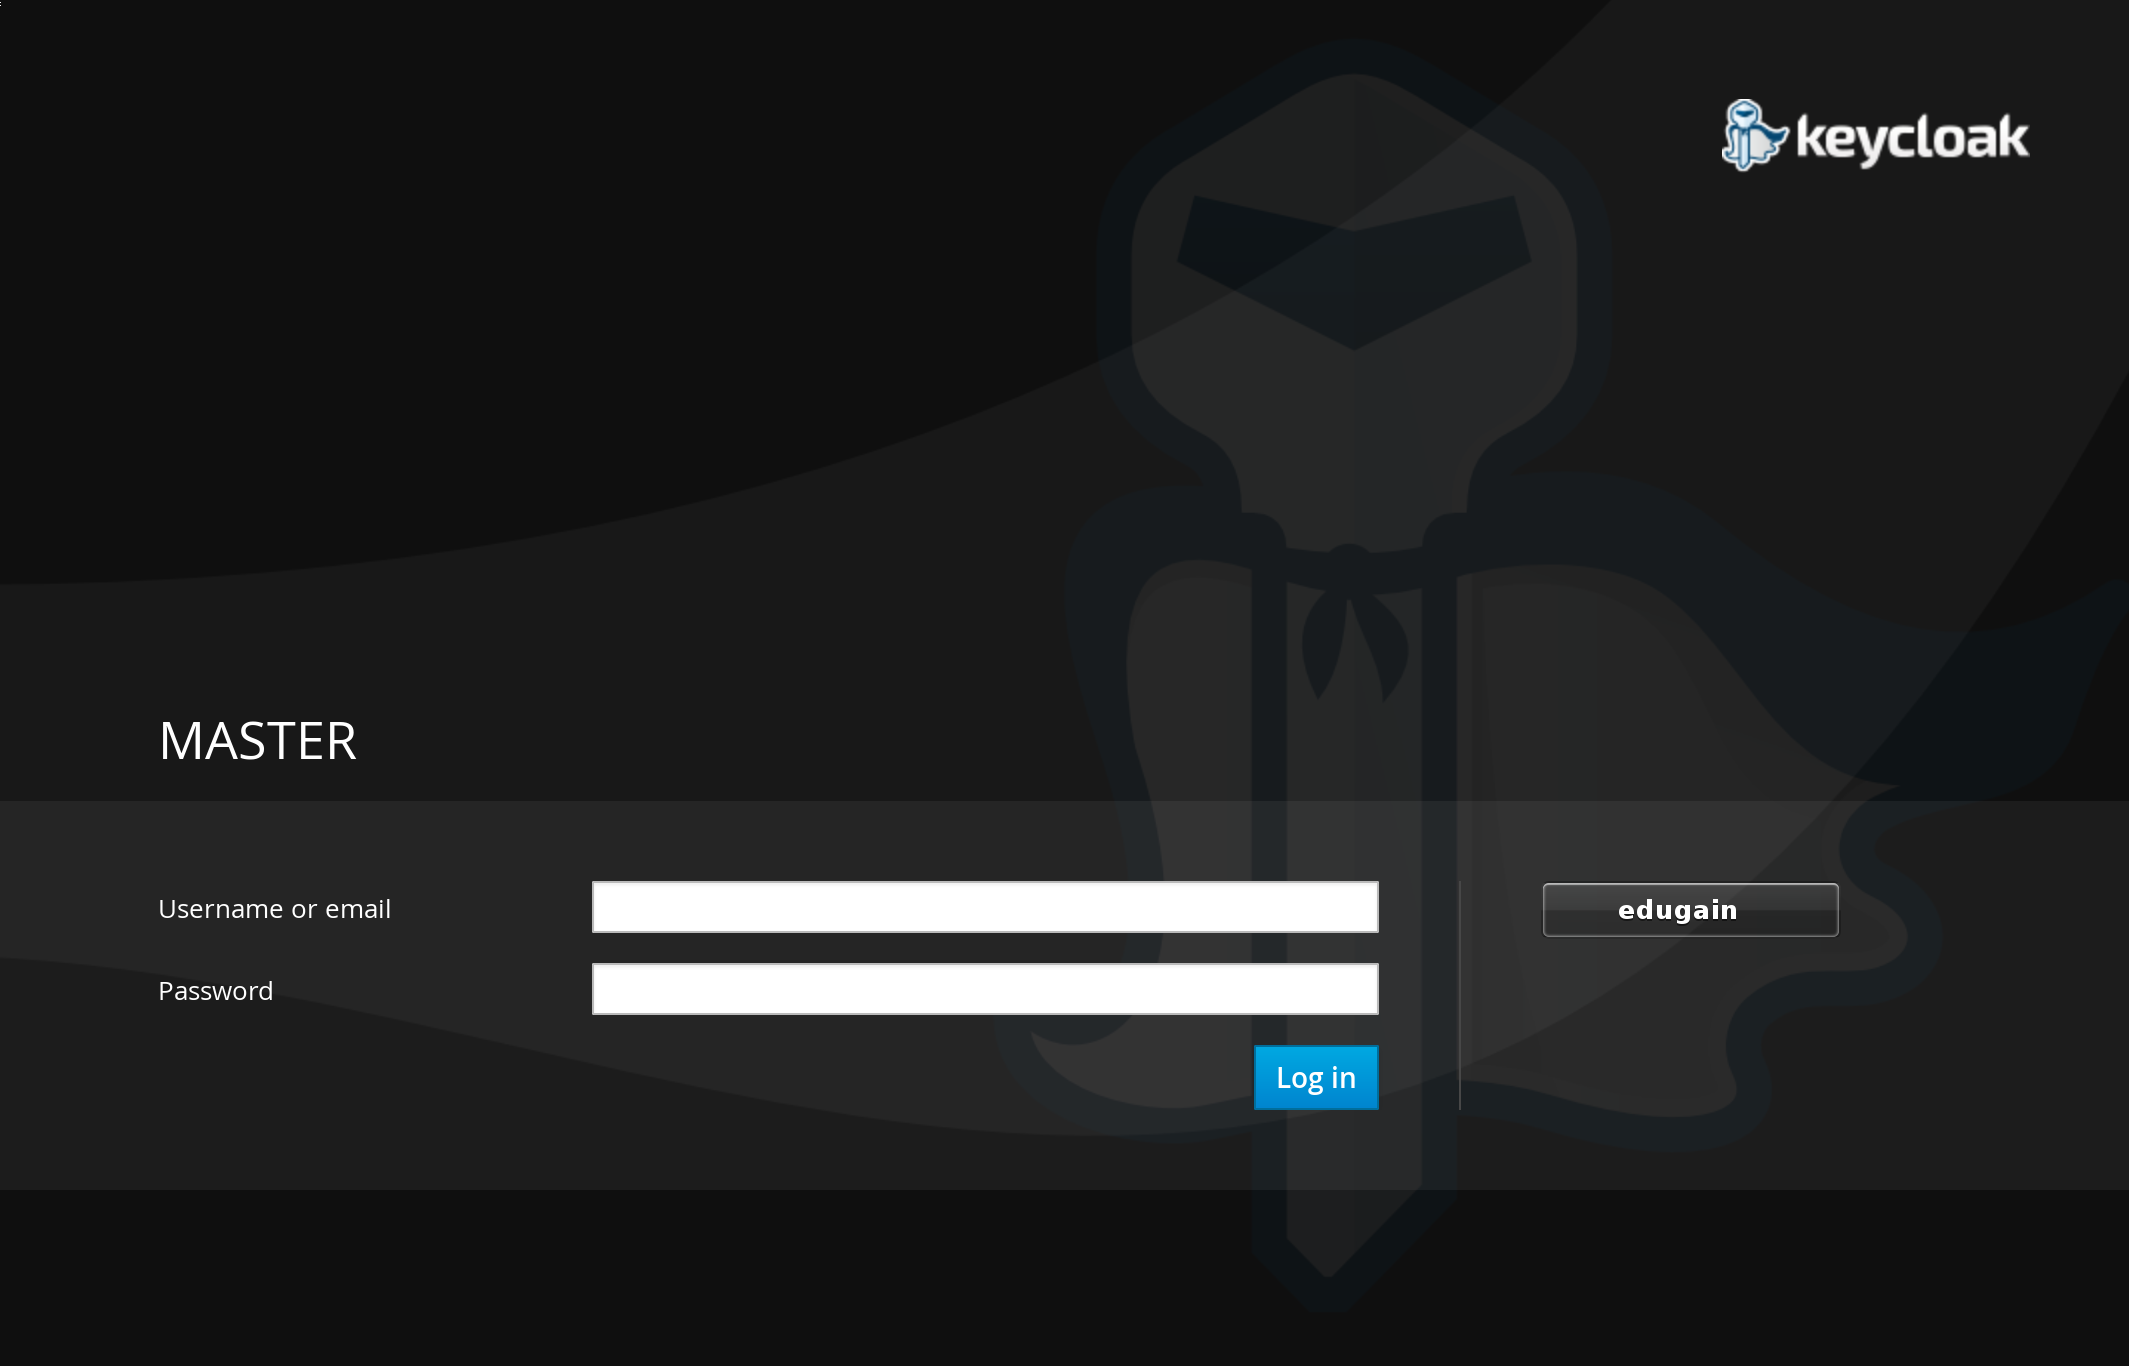
\includegraphics[width=\textwidth]{cyclone-federation-provider-login}\\
    Login screen to CYCLONE Federation Provider.
\end{center}


\vspace{0.5cm}

\section{Android}


\vspace{0.5cm}

\section{iOS}
